\section{Background} \label{sec:background}
The robotics association industry defines robotics as ``a robot is a re-programmable, multi-functional, manipulator designed to move material, parts, tools or specialised devices through variable programmed motions for the performance of a variety of task''. according to that definition any device that is programmed to preform variety of tasks is classified as a robot. Most of the robots consists of :
\begin{itemize}
	\item Physical body
	\item Actuators
	\item Sensors
	\item Controller
	\item Processor
	\item Software 
\end{itemize}
Those components are commonly used when designing and developing a robot. A good design is the one who best utilizes these components to reach it's goals effectively.
\subsection{Behaviours}
A robot Behaviour is defined by how it's motor action will be changed to perform a certain action according to it's sensor reading.Robots have three main control architecture:
\begin{itemize}
	\item Deliberative approach
	\item Reactive approach
	\item Hybrid approach (Deliberative and Reactive) 
\end{itemize}

The Deliberative approach requires high-level of intelligence and has slow response time. On contrary the reactive approach require simple processing and has real-time response. 
Designed behaviour of a report will require multiple function to be executed together. A combination of behavioural functions might not achieve the anticipated repose towards a change of the environment, to solve this problem a coordinator function is implemented to ensure correct behaviour of the robot. In designing coordination function there are two main strategies:
\begin{itemize}
	\item competitive: In which one behaviour overshadows any other behaviour and should be executed solely.
	\item cooperative: In which a collection of behaviour is executed to achieve a certain goal.
\end{itemize} 
Any Behavioural approach for robots is represented as a vector and to perform cooperative coordination between behaviours we use vectors addition. The main potential fields are uniform, perpendicular, attraction,repulsion and tangential. As Shown in {\ref{fig:Potential_fields}}:

\begin{figure}
\centering
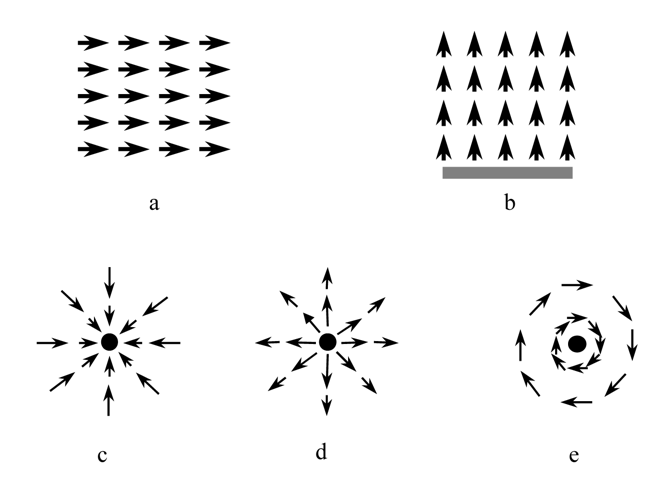
\includegraphics[width=0.7\linewidth]{figures/Potential_fields}
\caption{Five Main Potential Fields}
\label{fig:Potential_fields}
\end{figure}

%Make the list A B C instead of 1 2 3%
\begin{enumerate}
	\item Uniform means that robot will move in one direction.
	\item Perpendicular means that robot will move in a direction 90 degrees from the object.
	\item Attraction will make the object go towards the object.
	\item Repulsion the robot will move away from the object. \item Tangential when implemented will make the robot rotate and the edge of the object's perimeter. 
\end{enumerate}

\subsection{E-Puck}

\begin{figure}
\centering
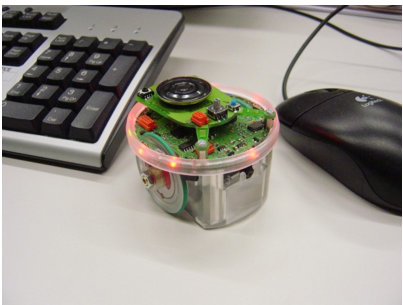
\includegraphics[width=0.7\linewidth]{figures/epcuk}
\caption{}
\label{fig:epcuk}
\end{figure}


E-Puck robots is a small size educational robot which is designed to be flexible and have a desktop size. It's also a low cost robot due to the choice of the components used. It's user-friendly and interactive. It was designed by Martin Stefanec from the artificial life lab of University of Graz \cite{epuck}. 

It includes a wide range of sensors and actuators. Sensors include infrared-sensors which can be used to detect objects and ambient light. Motors to control the movement of the robot. For visual communication the robot is has 8 LEDs and for audible communication it has a speaker.

\subsection{HSV}


HSV stands for Hue, Saturation and value. It's a cylindrical representation of colours, starting at red in 0 degrees, green at 120 degrees and blue at 240 degrees. the vertical axis which is value represents colours ranging from to neutral to black.

\begin{figure}
	\centering
	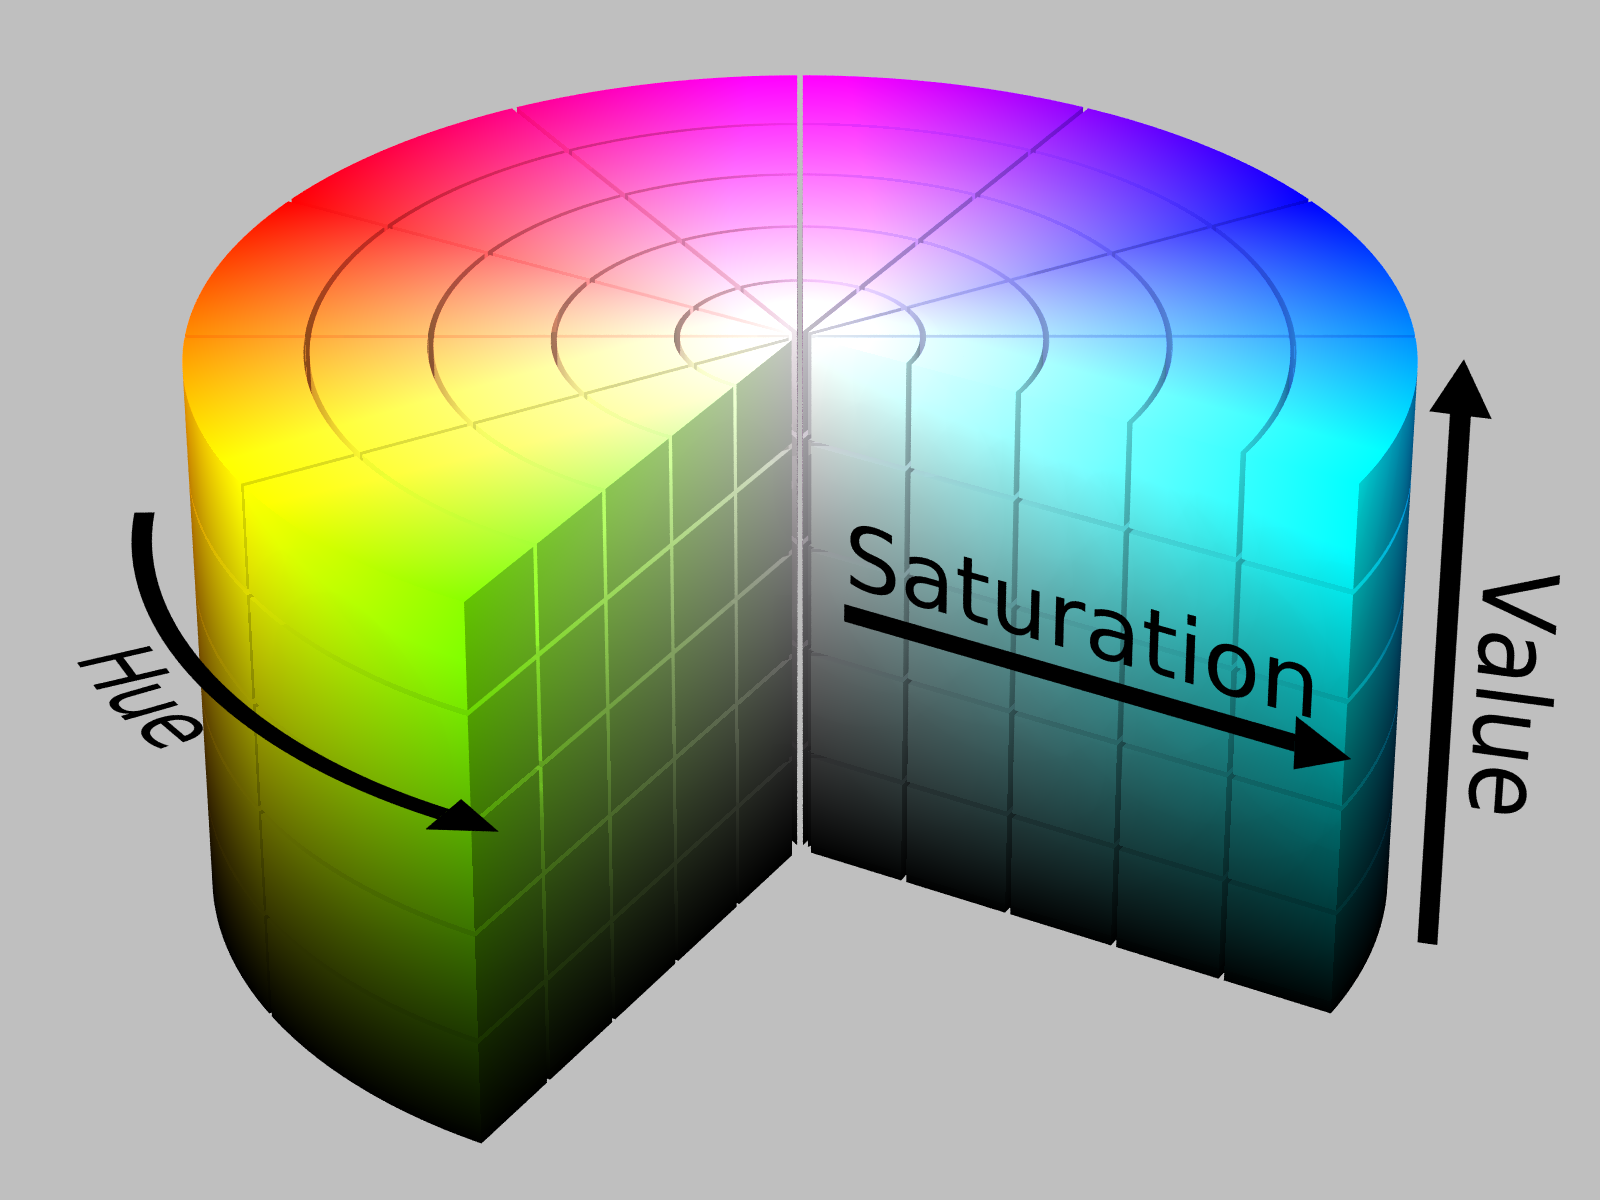
\includegraphics[width=0.7\linewidth]{figures/hsv}
	\caption{HSV Colour Space}
	\label{fig:hsv}
\end{figure}


\subsection{Skin Colour}

Skin detection in HSV tends to be more accurate than RGB. For efficient skin color detection RGB image is converted to HSV as HSV relates more to skin colour perception. In Hue skin colours varies from 0 to 50 degrees \cite{hsv_skin}. 
 